

\chapter{Introduction}



A cipher consist of en encoder and a decoder. The algorithm behind the encoder and the decoder has to be public in order to ensure the integrity and the robustness of the cipher. The ciphers are typically  open source projects, reviewed by security experts.  \\

\subsection{Definitions}

\begin{flalign*}
\emph{Encoder : }  &E : KxM \mapsto C  \\
\emph{Decoder : }  &D : KxC \mapsto M  \\ 
\emph{Equality : } &D(k, E(k,m) ) = m  
\end{flalign*}

E is often randomized whereas D is always deterministic. A cipher consist of the encoder and decoder : cipher $=$ $(E,D)$.



\begin{figure}[ht!]
	\centering
		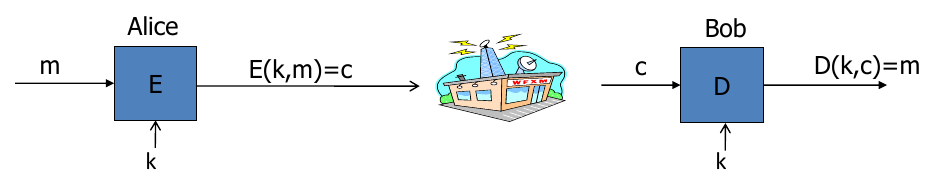
\includegraphics[width=0.7\textwidth]{images/tata}
	\caption{Cipher}
	\label{fig:Cipher}
\end{figure}

A common mistake is to think that an ad-hoc crypto algorithm with closed source is safer than open source standards : the big problem with closed source algorithms is that, when they are breached, the user does not know.\\


Uses of crypto : 
\begin{itemize}
		\item Secure communication : private conversations without eavesdropping 
		\item Digital signatures : secure identification (no tampering)
		\item Anonymous communication : secure and private communication without any of the participants know the identity of the others  
		\item Anonymous computation : outsourcing computation without giving the purpose of the calculus to the contractor (e.g. Amazon w3s)\\
\end{itemize}

\subsection{Trusted authority}

One way to ensure confidentiality is to outsource the task to a third party which has credibility and trust, like when we give our last will to a exterior person which does not have any involvement with the family(typically a \emph{notaire}).

However, the trusted authority solution - like any centralized mecanism -  creates a single point of failure, so the trusted authority might not be always a good solution. \\

\emph{Theorem} : Any computation done by trusted authority can be done without it.\\


\subsection{ Zero proof of knowledge }

\textit{Aim of cryptography} : prove that, under a certain threat vector, forge the signature comes to solve a NP-problem. \\

The definition of a NP-problem is that it is computationally "hard" to solve (nondeterministic polynomial time), but easy to verify a solution (called signature).

A zero-knowledge proof is a signature the user present to the server, which will answer true or false based on the signature's validity. Under zero-knowledge hypothesis, the user does not learn anything more than the validity of the signature.

\subsection{History of ciphers}

Cryptology is an ancient matter : all sorts of encoding scheme has been invented throughout History. \\


\emph{Definition :} $E(k,m)$ is the encryption of message $m$ using key $k$. (the key always first ) \\
\emph{Definition :} $D(k,c)$ is the decryption of ciphertext $c$ using key $k$. (the key always first ) 

\subsubsection{Substitution cipher }
The substitution cipher ( also called Caesar cipher in its weak form ) is a simple encoder, yet relatively effective : the key $K$ is a bijective map between two alphabets. For example, $A$ becomes $C$, $B$ becomes $O$, etc.\\

\begin{table}[ht!]
    \centering
    \scalebox{0.9}{
		\begin{tabular}{|c|c|c|c|c|c|c|c|c|c|c|c|c|c|c|c|c|c|c|c|c|c|c|c|c|c|c|}
			\hline
$input$&a&b&c&d&e&f&g&h&i&j&k&l&m&n&o&p&q&r&s&t&u&v&w&x&y&z \\
$output$&c&o&a&h&l&z&m&v&n&e&b&q&s&j&u&k&w&r&p&g&t&i&d&x&f&y \\
            \hline
		\end{tabular}
    }
	\caption{Substituion table}
	\label{tab:SubstitionTable}
\end{table}

Example of a encryption : 
\begin{alignat*}{3}
    &\text{plaintext}   & : & \text{ several flamethrowing sharks}&  \\
    & \downarrow        & : &   \downarrow & \\
    &\text{cyphertex}   & : & \text{ plilrcq   zqcslgvrudlr pvcrbp}&  \\ 
\end{alignat*}


The encryption is simply the substitution of every letter in the message $m$ by its counterpart in the map $K$.\\
The substitution cipher is however breakable just by looking at ciphertexts. The study of the letters' frequencies in the ciphertexts can give huge informations on the map $K$. In English, the letter "$e$" is the most used so, by looking which letter is the most used in the ciphertexts, we can give a pretty good guess of the subsitution of "$e$".\\

\begin{figure}[ht!]
    \centering
		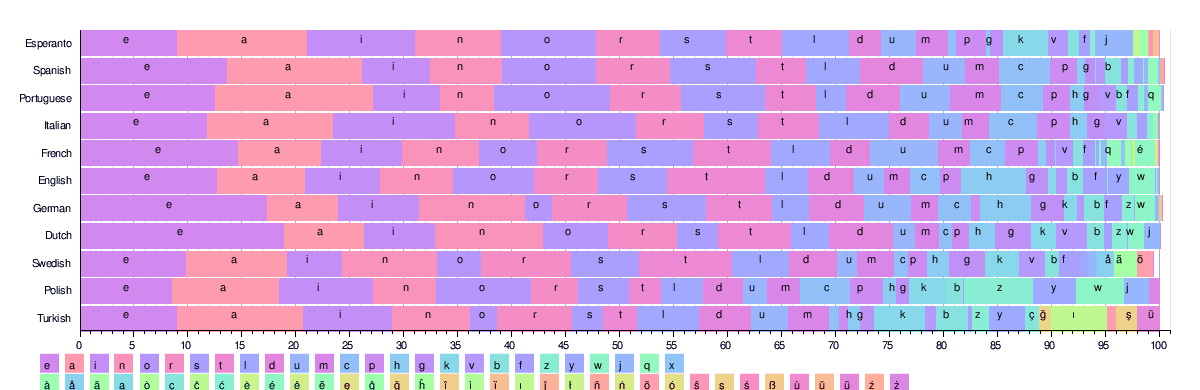
\includegraphics[width=\textwidth]{images/letter_frequency}
	\caption{Letter frequencies in several languages. It is fairly easy to guess the message's language just by looking at letter's repartition. \\ source : Wikipedia}
	\label{fig:LetterFrequency}
\end{figure}

The Caesar cipher is a simpler (and weaker) version of the substitution cipher : every character in the alphabet is offsetted by a constant value (modulo the alphabet's length). For example $A$ become $C$, $B$ become $D$, and so one... In this form, the key is not a map anymore, but only a constant integer,which is far smaller. 

\newpage
\begin{minipage}[c]{\linewidth}
    \lstinputlisting[
        language=Python,
        label= SubstitutionCode,
        caption=Substitution Code (in Python 2.7)
        ]{code/substitution.py}
\end{minipage}
\vfill


\subsubsection{ Vigenere cipher }

The  Vigenere cipher is built from the substitution code. The cipher use a work as key : every character will be used as a Caesar cipher encryption scheme. 
Example of a encryption : 
\begin{alignat*}{3}
    &\text{plaintext}   & : & \text{flamethrower}&  \\
    &\text{key}         & : & \text{vigenerecode}&  \\
    &\text{cyphertex}   & : & \text{ztgqrayvqkhv}&  \\ 
\end{alignat*}

If yhe encryption is based on a sum of letter position in the alphabet modulo the alphabet's length, the decryption is as simple since it's a difference: 

Example of a decryption : 
\begin{alignat*}{3}
    &\text{plaintext}   & : & \text{ztgqrayvqkhv}&  \\
    %&\text{plaintext} &:& \text{------------}&  \\
    &\text{key}         & : & \text{vigenerecode}&  \\
    %&\text{plaintext} &:& \text{____________}&  \\
    &\text{cyphertex}   & : & \text{flamethrower}&  \\ 
\end{alignat*}

\begin{figure}[ht!]
    \centering
        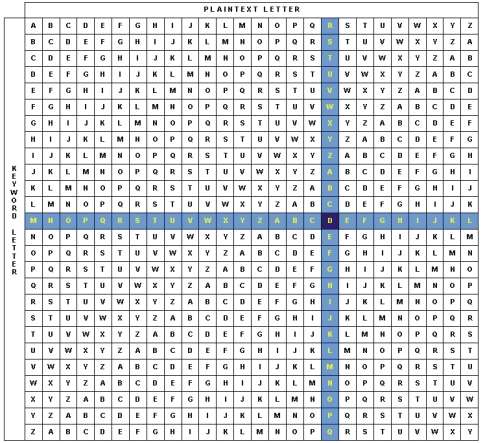
\includegraphics[width=0.7\textwidth]{images/vigenere}
	\caption{Vigenere \emph{tabula recta} for handmade encryption\\ source : illuminations.nctm.org}
	\label{fig:LetterFrequency}
\end{figure}

The Vigenere code is a fairly simple encryption scheme yet it were quite powerful (before the invention of automatic computation) since the encryption/decryption is a time-linear operation (table lookups) whereas the brute-force attack involve time-polynomial operations (multiple tables creation and lookups). It is still fairly easily breakable if the key's length is known to the attacker because it revert the cipher to a substitution one. Morevover, there are several methods which estimate the key's length based on frequency analysis (the vigenere cipher does mask all letter frequency patterns).\\





On a side note, if the key is smaller than the encoding message, they key is repeated and padded to match the message's length:
\begin{alignat*}{3}
    &\text{plaintext}   & : & \text{several flamethrowing sharks}&  \\
    %&\text{plaintext} &:& \text{+++++++ +++++++++++++ ++++++}&  \\
    &\text{plaintext}   & : & \text{smallsm allsmallsmall smalls}&  \\
    %&\text{plaintext} &:& \text{____________}&  \\ 
    &\text{cyphertex}   & : & \text{flamethrower}&  \\ 
\end{alignat*}


\subsubsection{Enigma}

The enigma machine is a device built by a German company around 1920 and consist of rotating substitution ciphers : 

\begin{figure}[ht!]
        \centering
        \begin{subfigure}[b]{0.4\textwidth}
                \centering
                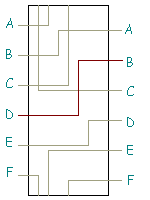
\includegraphics{images/enigma_rotor1}
                \caption{A is mapped to B}
                \label{fig:enigma_rotor1}
        \end{subfigure}
        \begin{subfigure}[b]{0.4\textwidth}
                \centering
                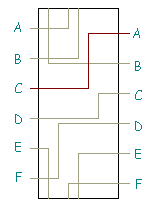
\includegraphics{images/enigma_rotor2}
                \caption{A is now mapped to C}
                \label{fig:enigma_rotor2}
        \end{subfigure}
        \caption{Enigma rotor : the rotor rotate by a increment for every new input, which lead to a different substitution table. \\ Source : www.bibmath.net }\label{fig:enigma_rotors}
\end{figure}

In order to strenghten the protocol, a typical Enigma machine use 3 rotors and a reflector\footnote{There is also a plugboard, which swap at most two pairs of letters.}. The reflector is a fixed rotor which acts as a mirror (it 's a simple substitution cipher) and each rotor is incremented by a special transition from the rotor on the left (apart from the most left one, which is incremented at each new input). In this configuration, the rotors' configurations act as public keys while the rotors' initial position as well as the rotors' order is the private one. The rotors can be sold or stolen without revealing anything about the encryption (apart from degenerate rotor configurations). The machine being symetrical, the cipher is symetric too : using the same private key, typing the ciphertext into the machine will print the plaintext message\footnote{Mathematical proof of the Enigma's symmetrical property can be found here : ??? .}.


\begin{figure}[ht!]
    \centering
        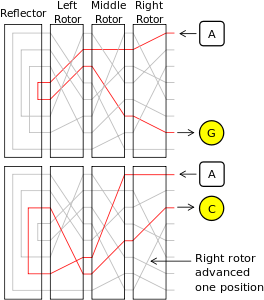
\includegraphics[width=0.7\textwidth]{images/Enigma_3rotors}
    \caption{ Enigma machine with 3 rotors and a reflector.\\ source : Wikipedia}
	\label{fig:enigma_3rotors}
\end{figure}

The enigma machines were largerly used during World War II by the German Army as a crypto-system. The breaking of Enigma di occupy a lot of mathematicians and logicians at that time, and bring numerous breakthroughs in cryptology. Finally, Alan Turing \footnote{also known as the most badass computer scientist of the 20th century} did crack the cipher using "crib" techniques : by analysing ciphertexts and some partial plaintexts (such as headers, known contents,...), it was possible to deduce the inner structure of the machine, and creating an automatic decypher called \emph{Bombe}.






